\begin{figure*}[!t]
\centering
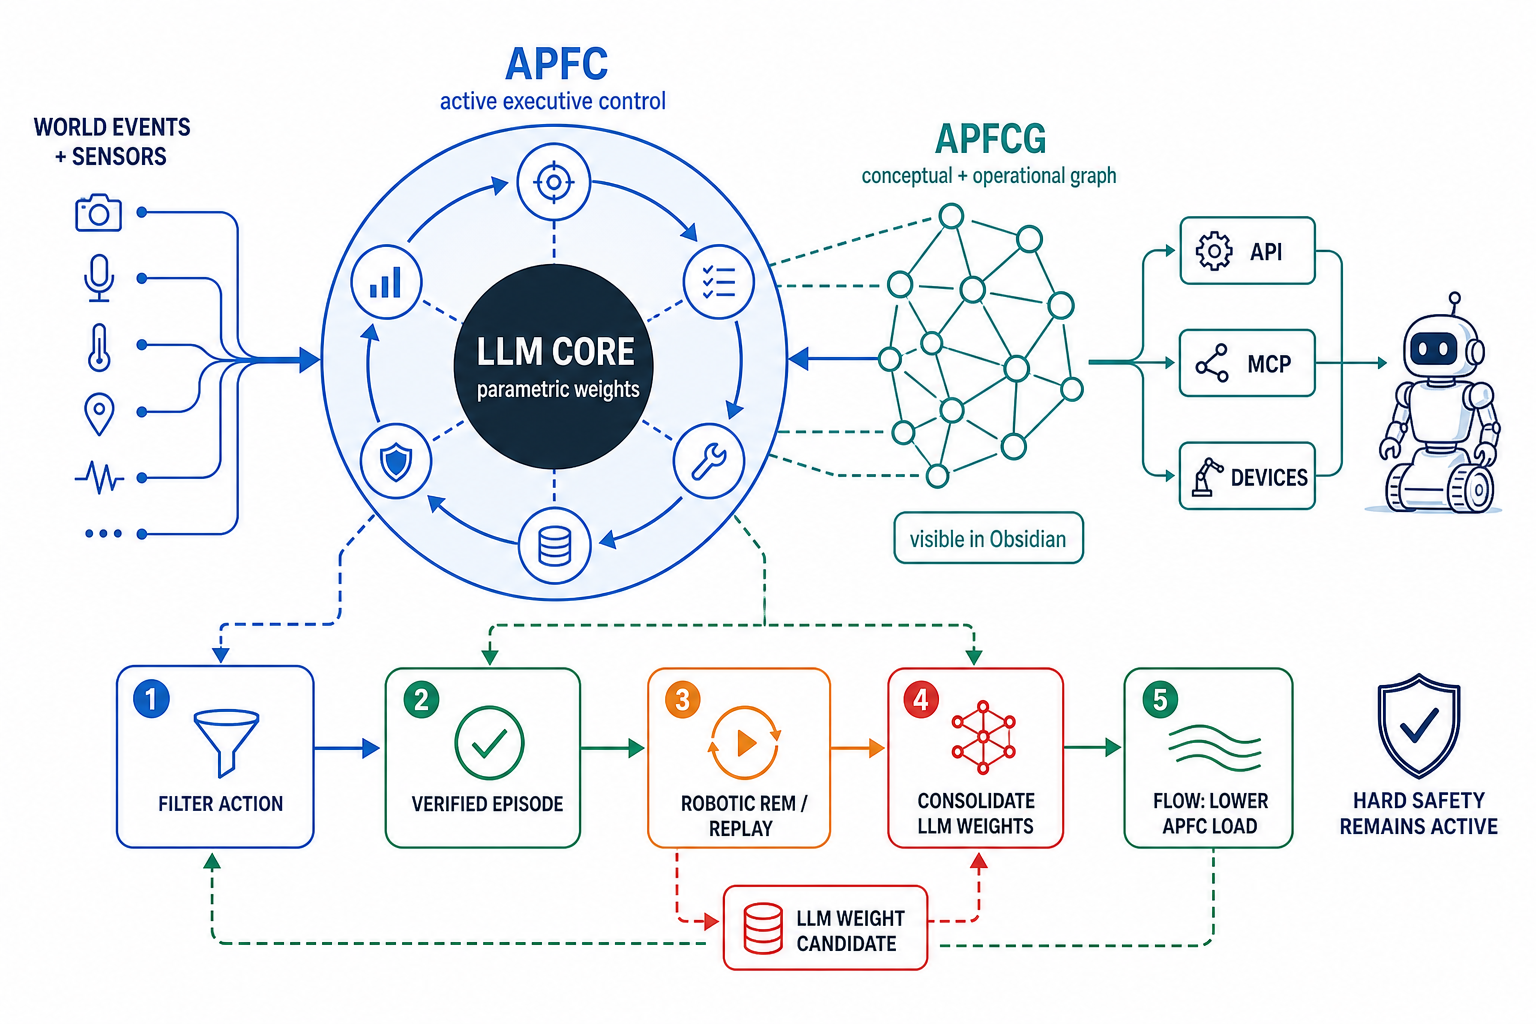
\includegraphics[width=0.98\textwidth]{figures/assets/md_os_apfc_apfcg_architecture_v2.png}
\vspace{0.35em}

\fbox{\begin{minipage}{0.94\textwidth}
\centering\small
\textbf{CORTEX = CODEX + MD-OS.}\quad
Codex here means the execution stack: OpenAI's local Codex CLI is open-source
Apache~2.0 software
(\href{https://github.com/openai/codex}{\nolinkurl{github.com/openai/codex}})
and mediates a selected external OpenAI model, tools, terminal, and bounded
read--write--execute loop.  The CLI source is open; this does not claim that
model weights or hosted services are open source.  MD-OS supplies the
persistent self-frame, executive method, APFC control, APFCG, policy, memory,
verification, and readback.\\[0.2em]
\textbf{EMBODIED LEARNING: ROBOT ACTS $\rightarrow$ WEBCAM OBSERVES THE ROBOT
$\rightarrow$ APFC LEARNS BODY--ACTION--EFFECT $\rightarrow$ APFC FILTERS THE
NEXT ACTION.}
\end{minipage}}
\caption{MD-OS CORTEX and the proposed wake--consolidation--flow cycle,
redrawn from the original project schema.  The central LLM weights are not the
whole agent.  In the implementation evaluated here, the functioning cortex is
the composition of the Codex execution stack---the open-source local CLI plus
a selected external model---and MD-OS, the persistent APFC operating
filesystem.  APFC is the active executive function;
APFCG is its durable heterogeneous graph.  APFCG links Markdown pages,
concepts, claims, and schemas; JSON/NDJSON state and evidence; application
workflows and action receipts; Python, JavaScript, PHP, shell, and other
bounded executors; and connectors to APIs and devices.  Obsidian visualizes
the linked-Markdown projection, not the whole graph or execution mechanism.
Because the robot is itself present in the sensory field, webcam feedback is
also self-observation: verified command-dependent bodily changes consolidate
an operational self-model that APFC uses to predict and filter later actions.
The lower cycle---robotic replay, candidate weight consolidation, sealed
promotion, and reduced APFC load during verified flow---is proposed; hard
safety remains active.}
\label{fig:apfc-apfcg-architecture}
\end{figure*}
